\chapter{CƠ SỞ LÝ THUYẾT}
\section{Học sâu và thị giác máy tính}
\subsection{Giới thiệu chung}

\begin{figure}[!h]
	\centering
	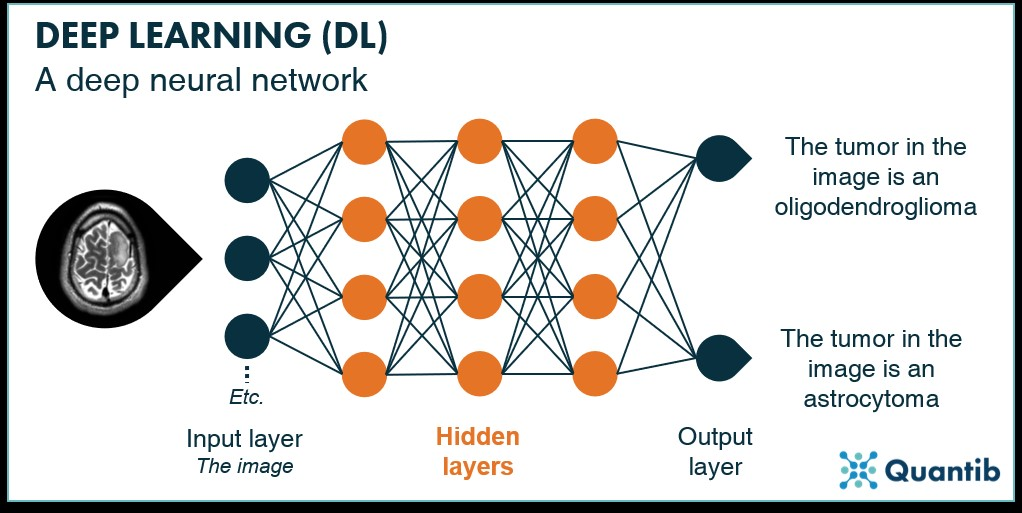
\includegraphics[width=100mm]{fig/DeepLearning.jpg}
        \captionsetup{justification=centering}
	\caption{Hình ảnh minh họa về Deep learning (nguồn Internet).}
	\label{fig_DL}
\end{figure}

Trong thời đại hiện nay, khả năng trí tuệ nhân tạo được cung cấp bởi các hệ thống thông minh dựa trên máy học (ML - machine learning) và học sâu đang ngày càng phổ biến. Máy học miêu tả khả năng của các hệ thống học tập từ lượng dữ liệu đào tạo để tự động hóa các quá trình phân tích mô hình và giải quyết các công việc liên quan \cite{janiesch2021machine}. Học sâu là một khái niệm dựa trên mạng Nơ-Ron nhân tạo và cho phép mô hình hóa các ứng dụng có yêu cầu cao hơn bằng cách sử dụng các cấu trúc mạng Nơ-Ron phức tạp hơn so với các mô hình học máy thông thường.

Học sâu (Deep Learning) là một phân nhánh của máy học và đã mang lại những tiến bộ đáng kể trong nhiều lĩnh vực nhờ vào khả năng xử lý lượng lớn dữ liệu và tự động hóa quá trình học tập. Các mô hình học sâu sử dụng mạng Nơ-Ron nhân tạo với nhiều lớp (multi-layer neural networks), cho phép chúng học được các đặc trưng phức tạp từ dữ liệu. Điều này giúp học sâu vượt trội trong các ứng dụng như nhận dạng hình ảnh, xử lý ngôn ngữ tự nhiên, và dự đoán xu hướng. Sự khác biệt quan trọng của học sâu so với các phương pháp khác là sử dụng mạng Nơ-Ron nhân tạo để tự động hóa việc đào tạo. Bằng cách sử dụng số lượng lớn dữ liệu đầu vào, học sâu có khả năng đào tạo mô hình tự động và tạo ra kết quả chính xác hơn so với phương pháp truyền thống của học máy.

Sự phát triển của AI, đặc biệt là học sâu, đã thay đổi cách chúng ta tiếp cận và giải quyết các vấn đề phức tạp. Từ chăm sóc sức khỏe, tài chính, đến giao thông và giải trí, AI đang dần trở thành một phần không thể thiếu, đem lại những cải tiến và tối ưu hóa vượt bậc cho nhiều lĩnh vực khác nhau. Nhờ vào AI, chúng ta có thể kỳ vọng vào một tương lai nơi công nghệ không chỉ hỗ trợ mà còn nâng cao chất lượng cuộc sống con người theo những cách chưa từng có.

\subsection{Mạng nơ-ron nhân tạo}

\begin{figure}[!h]
	\centering
	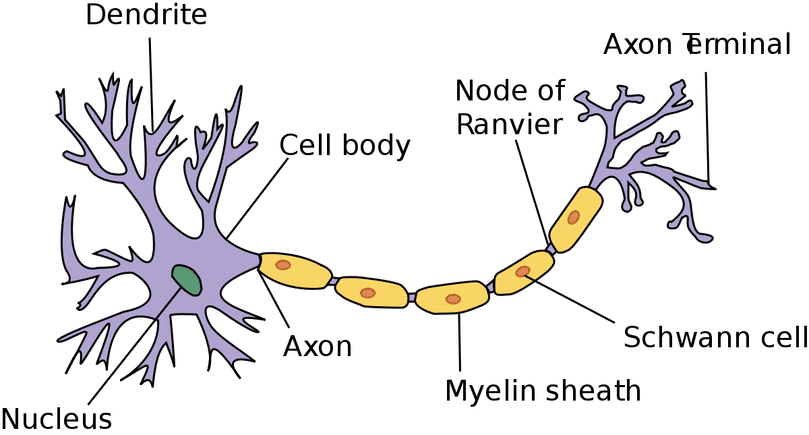
\includegraphics[width=120mm]{fig/notron.png}
        \captionsetup{justification=centering}
	\caption{Mô hình mạng Nơ-Ron (nguồn Internet).}
	\label{fig_Noron}
\end{figure}

Khái niệm Nơ-Ron là một đơn vị thần kinh được liên kết với hàng triệu đơn vị Nơ-Ron khác tạo nên một hệ thống thần kinh phức tạp và hoạt động bằng cách nhận dữ liệu từ đầu vào của nó và truyền đi cho các Nơ-Ron khác trong hệ thống. Ngày nay, DL dựa trên cách hoạt động của mạng Nơ-Ron thần kinh để xây dựng lên một hệ thống mạng thần kinh gồm các lớp Nơ-Ron nhân tạo và bắt chước theo các tính năng của nó để áp dụng vào trong lĩnh vực trí tuệ nhân tạo (AI – Artificial Intelligence). Từ đó mô hình mạng Nơ-Ron ra đời và giúp cho lĩnh vực AI phát triển một cách vượt bậc nhờ khả năng suy luận gần giống như hành vi của con người. Nói cách khác mô hình mạng Nơ-Ron nhân tạo cố gắng mô phỏng lại gần chính xác với quy trình xử lý thông tin như là bộ não của con người.

Trong mạng nơ-ron nhân tạo, các nơ-ron được tổ chức thành các lớp bao gồm lớp đầu vào (input layer), lớp ẩn (hidden layers) và lớp đầu ra (output layer). Mỗi lớp có nhiệm vụ chuyển đổi và truyền tải thông tin theo một cách thức nhất định. Nhờ vào quá trình học (training), trong đó mạng nơ-ron điều chỉnh các trọng số dựa trên dữ liệu đầu vào và đầu ra mong muốn, mạng nơ-ron nhân tạo có thể học hỏi từ dữ liệu và đưa ra các dự đoán hoặc quyết định giống như cách con người học từ kinh nghiệm. Điều này giúp chúng có khả năng giải quyết các vấn đề phức tạp như nhận dạng hình ảnh, xử lý ngôn ngữ tự nhiên và chơi trò chơi, đưa lĩnh vực trí tuệ nhân tạo tiến xa hơn bao giờ hết.


\subsection{Sự khác nhau giữa học sâu, học máy và trí tuệ nhân tạo}


Thay vì hệ thống hóa kiến thức vào máy tính, ML sẽ tìm cách tự động học các mối quan hệ và mẫu có ý nghĩa từ các ví dụ và quan sát. Những tiến bộ trong ML đã cho phép sự gia tăng gần đây của các hệ thống thông minh với khả năng nhận thức giống như con người, thâm nhập vào công việc kinh doanh và cuộc sống cá nhân của chúng ta, đồng thời định hình các tương tác được kết nối mạng trên thị trường điện tử theo mọi cách có thể.

\begin{figure}[!h]
	\centering
	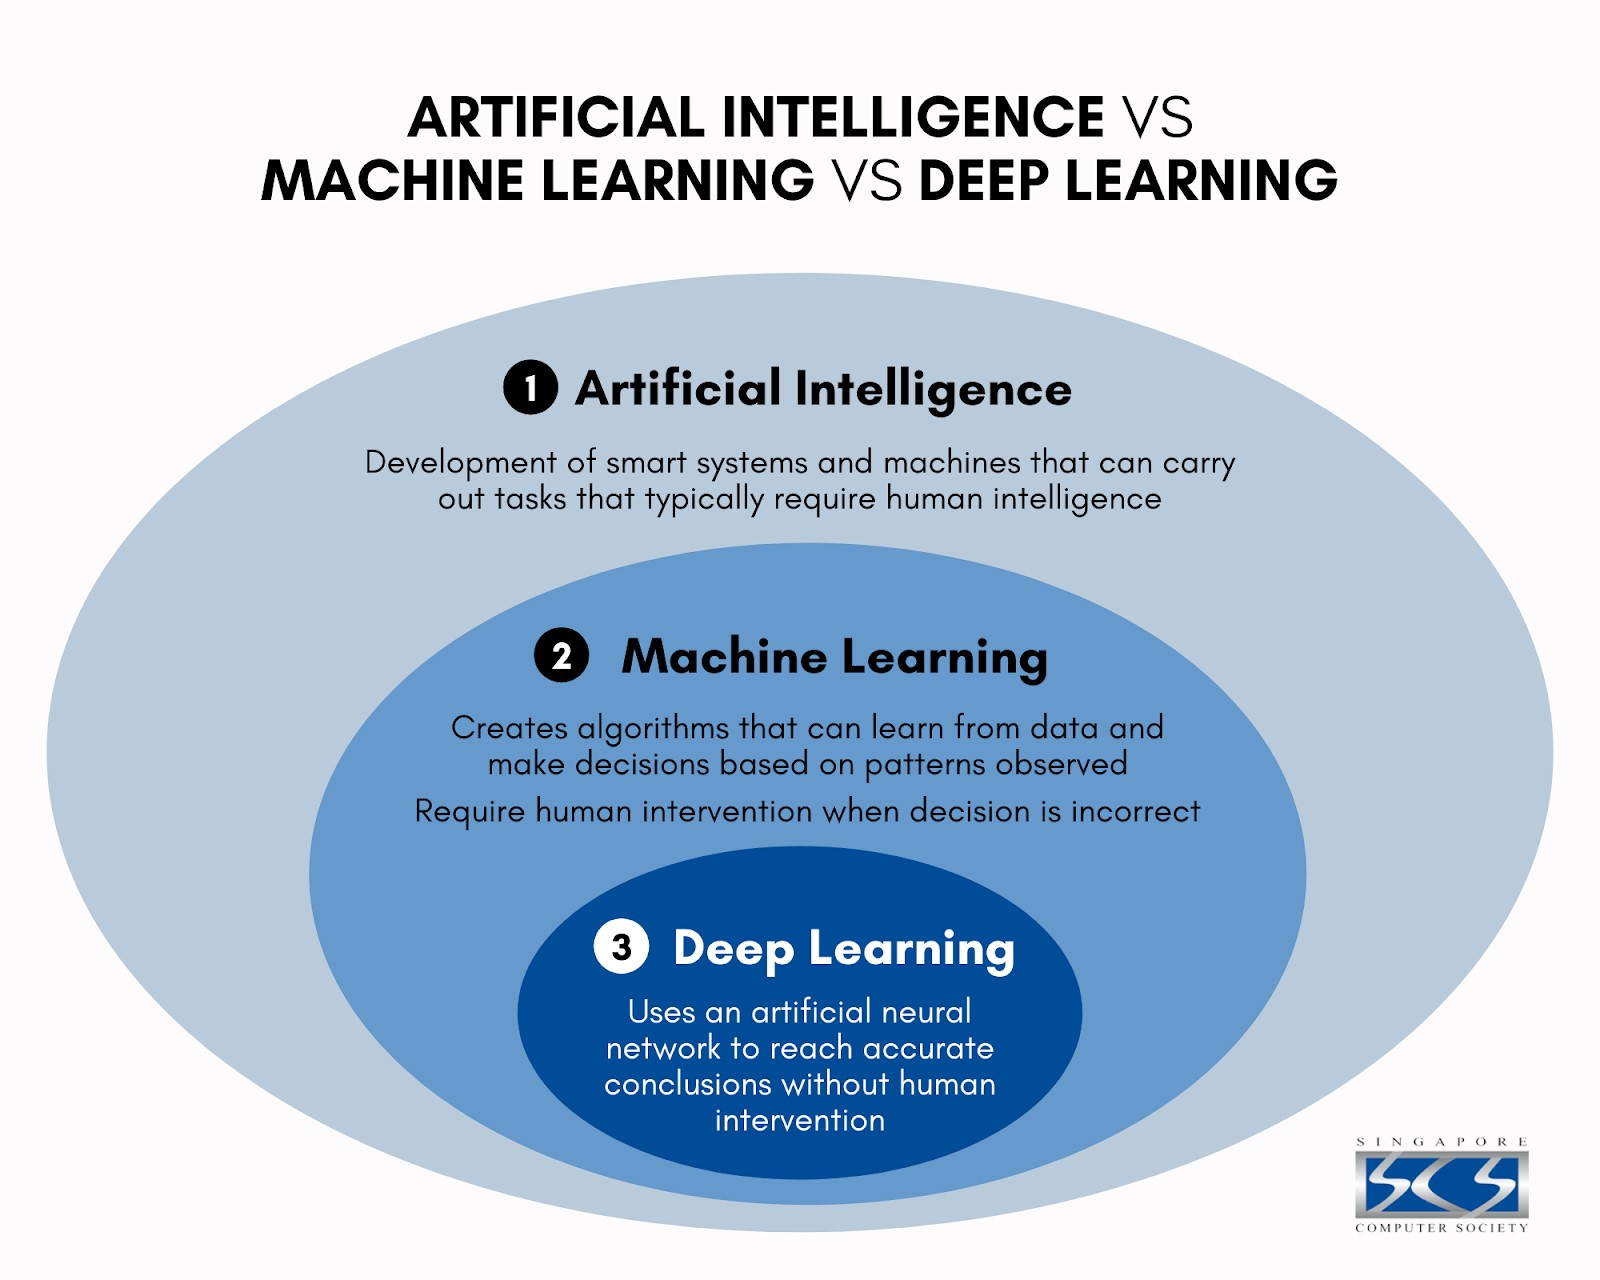
\includegraphics[width=100mm]{fig/AI_hierachical.jpg}
        \captionsetup{justification=centering}
	\caption{Mô hình phân cấp AL, ML, DL (nguồn Internet).}
	\label{fig_AL_hierachical}
\end{figure}

Các hệ thống ML và DL phức tạp hay còn được gọi là trí tuệ nhân tạo, nhờ khả năng xử lý và giải quyết các vấn đề phức tạp, phụ thuộc vào các mô hình phân tích và dự đoán các quy tắc để đưa ra câu trả lời hoặc đề xuất kết quả tương tự như con người. AI đã đóng góp vai trò quan trọng dựa trên việc giảm gánh nặng tính toán và dự đoán cho con người trong nhiều ứng dụng cụ thể. Tóm lại lĩnh vực trí tuệ nhân tạo phát triển phụ thuộc vào các mô hình DL và ML trong đó khái niệm về DL là một phương pháp được nâng cấp từ phương pháp học của ML trước đó bằng việc áp dụng mô hình mạng Nơ-Ron nhân tạo vào để xử lý các bài toán với cách thức tương tự như con người.

Từ đó lĩnh vực AI đã tạo ra nhiều tiến bộ trong ngành máy tính nói riêng và các lĩnh vực liên quan khác nói chung. Một trong những tiến bộ này là sự phát triển và ra đời của các mạng thần kinh Nơ-Ron nhân tạo từ đó khái niệm DL được ra đời \cite{janiesch2021machine}. Đối với các ứng dụng cụ thể như nhận diện vật thể hoặc phân loại đối tượng, việc ứng dụng DL đem lại nhiều hiệu quả vượt trội nhờ vào cách huấn luyện đặc biệt thông qua mạng thần kinh Nơ-Ron nhân tạo. Bằng cách trích xuất ra những đặc trưng của vật thể tại từng lớp mạng Nơ-Ron nhân tạo và điều chỉnh các trọng số sau mỗi chu kỳ huấn luyện cho đến khi tỷ lệ dự đoán đạt được là cao nhất.

\begin{figure}[!h]
	\centering
	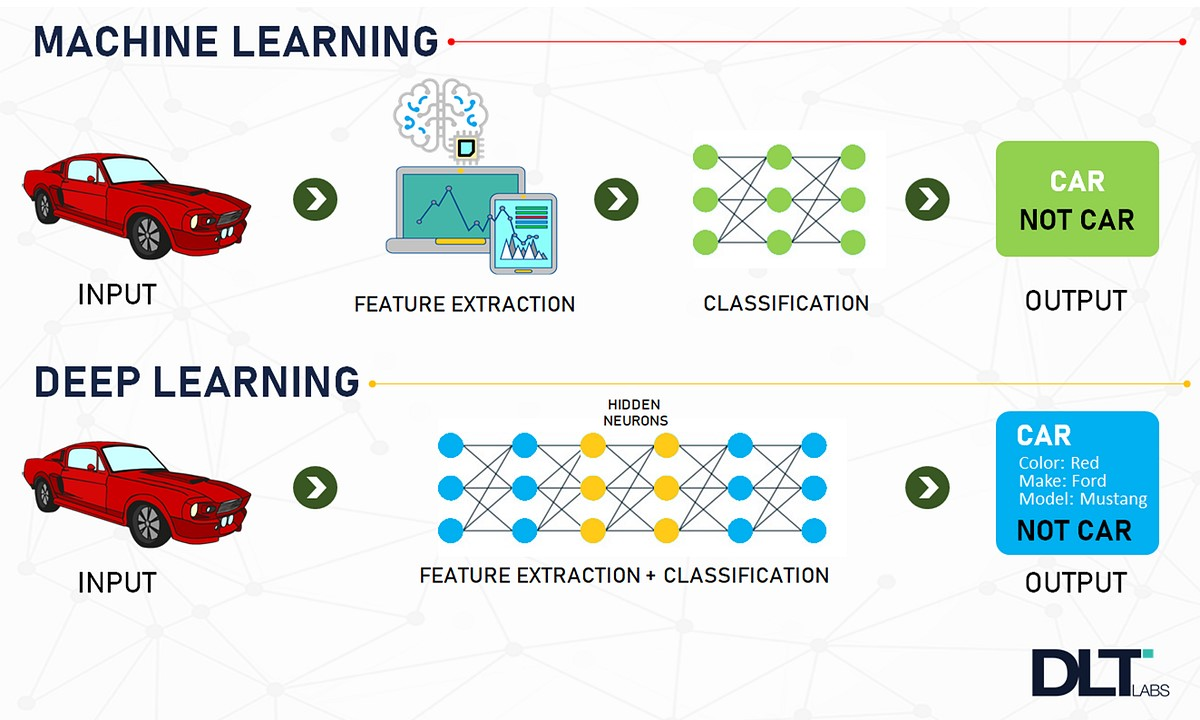
\includegraphics[width=100mm]{fig/DlandML.jpg}
        \captionsetup{justification=centering}
	\caption{Deep learning và Machine learning (nguồn Internet).}
	\label{fig_DlandML}
\end{figure}

Trong DL nguồn dữ liệu đầu vào là cơ sở giúp cho mô hình có thể bắt đầu quá trình học. Dữ liệu có thể là các đoạn văn bản, hình ảnh, biểu tượng và những dữ liệu đó được gọi là các dữ liệu chưa được xử lý. Khi dữ liệu đã được xử lý hay còn gọi là gắn nhãn thì nó được gọi là các thông tin và DL sẽ dựa vào các thông tin đó để ghi nhớ hình dạng cũng như các đặc điểm của vật thể từ đó điều chỉnh các trọng số phù hợp để đưa ra các dự đoán chính xác. Từ sự phát triển của DL đã mở ra khả năng xử lý được nhiều vấn đề thực tế và đưa các hành vi của máy tính trở lại gần giống với cách con người suy luận. Từ đó lĩnh vực AL đã được mở rộng và bao quát hơn nhờ DL.  


\section{Mô hình mạng CNN}
\subsection{Giới thiệu chung}

% Mô hình mạng CNN (Convolutional Neural Networks) là mạng tích chập được ứng dụng phổ biến trong các mô hình ứng dụng dùng để nhận diện và phân loại hình ảnh. Mô hình mạng CNN được ứng dụng rộng rãi trong các ứng dụng nhận diện và phân loại hình ảnh bằng cách sử dụng nhiều lớp tích chập, mỗi lớp tích chập sẽ trích xuất ra các đặc trưng của ảnh.

% Mô hình mạng CNN cơ bản sử dụng các lớp tích chập (Convolution layer) và các lớp tổng hợp (Pooling layer) chồng lên nhau để trích xuất ra các đặc trưng của ảnh đầu vào. Lớp tích chập đóng vai trò trích xuất ra các đặc trưng của ảnh đầu vào bằng cách sử dụng các mặt nạ (kernels) để lướt trên từng điểm ảnh và sử dụng phép nhân chập để trích xuất ra các thông số đặc trưng của ảnh đầu vào. Lớp tổng hợp đóng vai trò tổng hợp lại các tính chất của ảnh từ lớp tích chập và loại bỏ đi các tính chất không cần thiết và đưa ra kết quả.

Mạng nơ-ron tích chập, hay còn gọi là CNN (convolutional neural networks), là một loại mô hình mạng thần kinh nhân tạo đặc biệt được thiết kế để xử lý dữ liệu dạng lưới như hình ảnh. Được áp dụng rộng rãi trong lĩnh vực nhận diện và phân loại hình ảnh, CNN đã trở thành công cụ quan trọng và không thể thiếu trong nhiều ứng dụng thực tế.

Điểm mạnh của CNN nằm ở khả năng học và trích xuất các đặc trưng quan trọng của hình ảnh thông qua việc sử dụng các lớp tích chập (convolutional layers). Mỗi lớp tích chập trong mạng CNN có khả năng phát hiện và nắm bắt các mẫu (patterns) khác nhau trong dữ liệu đầu vào, từ các đặc trưng cơ bản như cạnh và góc, đến các đặc trưng phức tạp hơn như hình dạng và kết cấu. Quá trình này diễn ra thông qua việc sử dụng các bộ lọc (filters) và phép tích chập, giúp CNN có khả năng phát hiện các đặc trưng không gian trong ảnh một cách hiệu quả. Ngoài ra, CNN còn sử dụng các lớp pooling để giảm kích thước không gian của các đặc trưng đã được trích xuất, giúp giảm thiểu số lượng tham số và tính toán trong mô hình, đồng thời tăng khả năng tổng quát hóa của mô hình. Các lớp kết nối toàn phần (fully connected) ở cuối mạng đảm nhận vai trò phân loại dựa trên các đặc trưng đã được trích xuất và tổng hợp qua các lớp trước đó.

Nhờ vào cấu trúc đặc biệt và khả năng học hỏi mạnh mẽ, CNN đã được ứng dụng trong nhiều lĩnh vực khác nhau, từ y tế, như phát hiện và chẩn đoán bệnh qua hình ảnh y học, đến các ứng dụng trong xe tự lái, nhận diện khuôn mặt, phân loại đối tượng trong hình ảnh, và thậm chí là trong nghệ thuật số và truyền thông.

\subsection{Kiến trúc mạng CNN}

\begin{figure}[h]
	\centering
	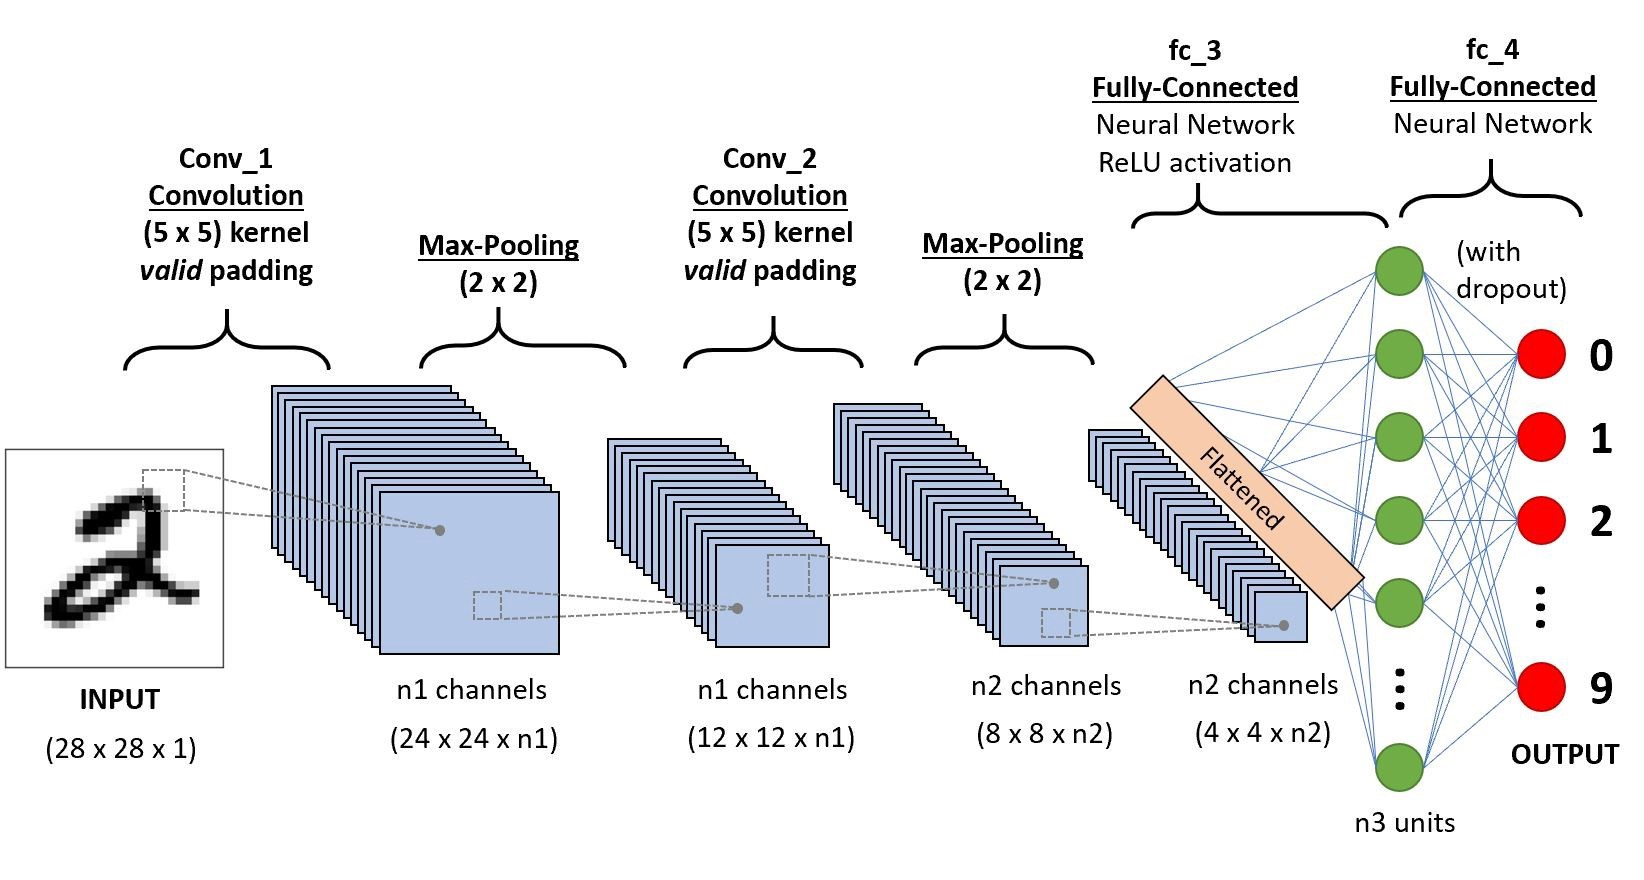
\includegraphics[width=120mm]{fig/CNNarchitecture.jpg}
        \captionsetup{justification=centering}
	\caption{Kiến trúc mạng CNN (nguồn Internet).}
	\label{fig_CNNarchitecture}
\end{figure}

Kiến trúc của mạng CNN được xây dựng dựa trên các lớp cơ bản như lớp tích chập (Convolution layer), lớp kích hoạt (RELU layer), lớp tổng hợp (Pooling layer) và lớp kết nối đầy đủ (Fully connected layer).

\begin{itemize}
    \item \textbf{Lớp tích chập (Convolution layer):} Lớp tích chập được coi là có vai trò quan trọng nhất trong kiến trúc mạng CNN, ở lớp này sẽ thực hiện các quá trình tính toán như nhân chập ảnh với mặt nạ (kernels), bộ lọc (filter), trích xuất đặc trưng (feature map). Trích xuất đặc trưng là yếu tố quan trọng nhất trong lớp tích chập.

    \item \textbf{Lớp Kích hoạt (RELU layer):} Lớp kích hoạt dùng để tính toán và mô phỏng lại tỷ lệ truyền xung qua axon của hệ Nơ-Ron thần kinh dùng các hàm kích hoạt (activation function) như leaky, mish, swish, v.v.

    \item \textbf{Lớp tổng hợp (Pooling layer):} Lớp tổng hợp sẽ lượt bỏ đi các thông tin không cần thiết từ lớp tích chập từ đó cho ra kết quả mong muốn.

    \item \textbf{Lớp kết nối đầy đủ (Fully connected layer):} Tại lớp kết nối đầy đủ sẽ lấy kết quả đầu vào từ lớp trước đó và tiến hành nén thông tin ảnh về dưới dạng một véc tơ và dùng kết quả đó để làm đầu vào cho lớp kế tiếp.
    
\end{itemize}

\subsection{Phép tích chập (convolution}

\begin{figure}[h]
	\centering
	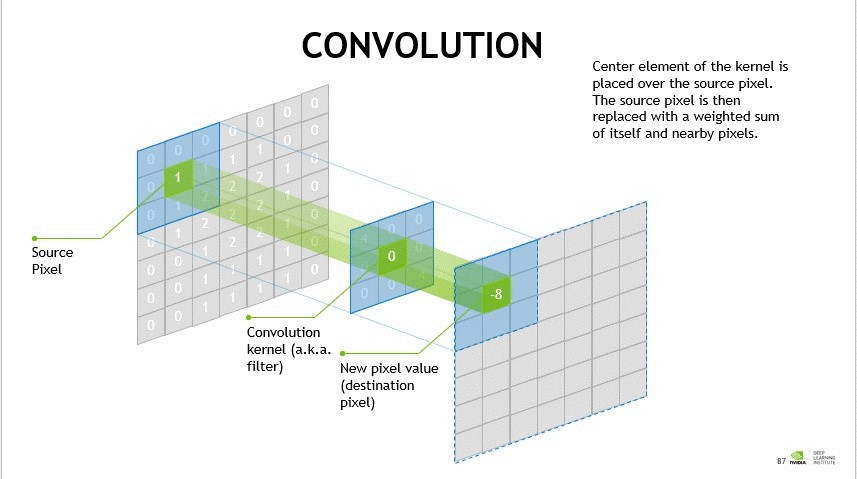
\includegraphics[width=120mm]{fig/eqconvolution.jpg}
        \captionsetup{justification=centering}
	\caption{Phép tính tích chập trên ma trận ảnh (nguồn Internet).}
	\label{fig_eqconvolution}
\end{figure}

\begin{equation}
    \mathrm{f(x,y) \ast k(x,y) = \sum_{u=-m/2}^{m/2} \sum_{v=-n/2}^{n/2} k(u,v) f(x-u,y-v)},
    \label{eq:convolution}
\end{equation}

Phép tích chập là một trong những phép toán quan trọng trong lĩnh vực xử lý ảnh, bằng cách sử dụng các mặt nạ để lướt trên từng điểm ảnh và tính tích chập tại từng điểm ảnh. Công thức tính phép tích chập tại một điểm ảnh $\mathrm{f(x,y)}$ với mặt nạ $\mathrm{k(x,y)}$ được biểu diễn tại (\ref{eq:convolution}). Phép tích chập có thể được hình dung như bằng cách dùng mặt nạ $\mathrm{K}$ dịch chuyển trên từng điểm ảnh từ góc bên của trái ảnh theo hàng ngang và theo hàng dọc khi đi tới điểm ngoài cùng bên phải của ảnh. Tương ứng với mỗi lần dịch chuyển sẽ thực hiện tính toán giá trị tại điểm ảnh đang xét bằng công thức tính phép tích chập.

\section{Phương pháp phân vùng ảnh}
\subsection{Giới thiệu về phương pháp phân vùng ảnh}


Phân đoạn hình ảnh~\cite{minaee2021image} là một nhiệm vụ quan trọng trong thị giác máy tính và xử lý hình ảnh, liên quan đến việc chia nhỏ các hình ảnh thành các đoạn hoặc đối tượng riêng biệt. Quá trình này là nền tảng cho nhiều ứng dụng khác nhau như hiểu cảnh, phân tích hình ảnh y tế, nhận thức robot, giám sát video, thực tế tăng cường và nén hình ảnh. 

\begin{figure}[h]
	\centering
	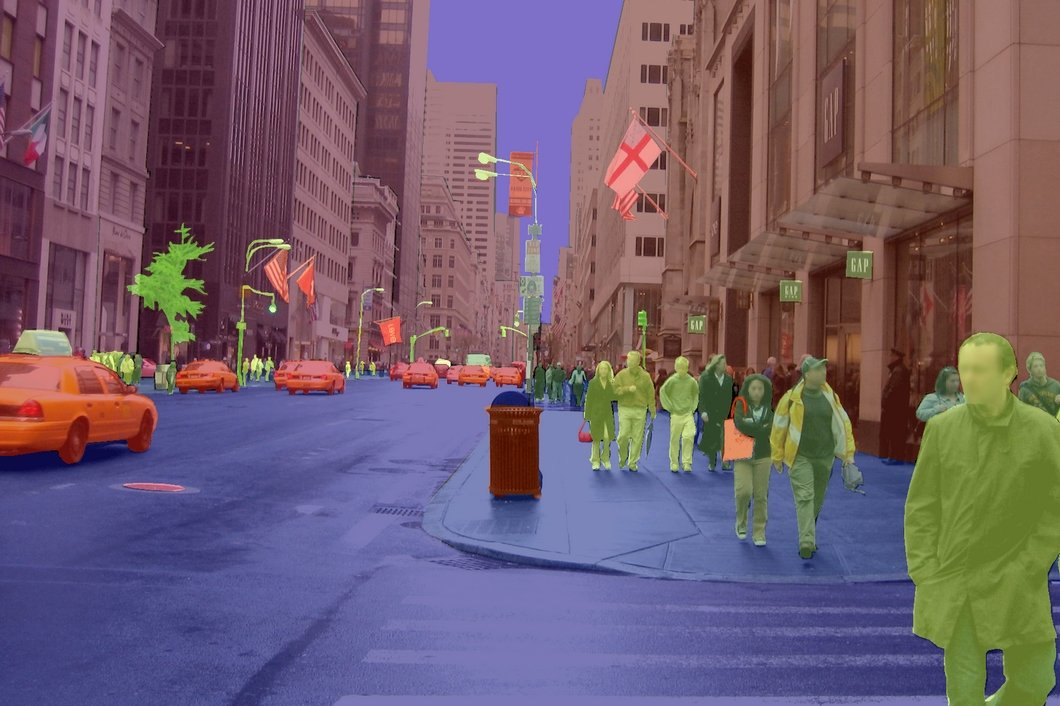
\includegraphics[width=120mm]{fig/image_segmentation.jpg}
        \captionsetup{justification=centering}
	\caption{Ví dụ về phân đoạn ảnh (nguồn Internet).}
	\label{fig_CNNarchitecture}
\end{figure}


Mục tiêu cơ bản của phân đoạn hình ảnh là đơn giản hóa hoặc thay đổi đại diện của một hình ảnh thành một cái gì đó có ý nghĩa hơn và dễ dàng phân tích hơn. Nó có thể được phân loại thành ba loại chính: phân đoạn ngữ nghĩa, phân đoạn đối tượng và phân đoạn tổng hợp. Phân đoạn ngữ nghĩa liên quan đến việc gán nhãn cho từng điểm ảnh của hình ảnh với một lớp tương ứng như 'xe hơi', 'cây cối' hoặc 'đường phố'. Phân đoạn đối tượng tiến xa hơn bằng cách xác định các đối tượng riêng lẻ, trong khi phân đoạn tổng hợp kết hợp cả phân đoạn ngữ nghĩa và phân đoạn đối tượng, cung cấp một sự hiểu biết toàn diện về cảnh.



\subsection{Một số phương pháp phân vùng ảnh}

Trong quá khứ, nhiều phương pháp khác nhau đã được sử dụng cho phân đoạn hình ảnh~\cite{minaee2021image}, bao gồm phân ngưỡng, phát triển vùng, các phương pháp phân cụm như k-means, và các kỹ thuật tinh vi hơn như các đường viền hoạt động và cắt đồ thị. Tuy nhiên, sự xuất hiện của học sâu đã thay đổi đáng kể lĩnh vực này, giới thiệu các mô hình tận dụng các mạng nơ-ron tích chập (CNN), các kiến trúc mã hóa-giải mã, mạng nơ-ron hồi tiếp và mạng đối kháng tạo sinh (GAN) để đạt được kết quả tiên tiến nhất. 

Các phương pháp phân đoạn hình ảnh dựa trên học sâu đã vượt trội hơn các phương pháp truyền thống, đạt được độ chính xác và hiệu quả cao hơn. Ví dụ, các mạng tích chập hoàn toàn (FCN - fully connected network) đã có vai trò then chốt trong cuộc cách mạng này, cho phép huấn luyện và dự đoán từ đầu đến cuối cho phân đoạn ngữ nghĩa. Các mạng này thay thế các lớp hoàn toàn kết nối trong các CNN truyền thống bằng các lớp tích chập duy trì thông tin không gian, cho phép mạng tạo ra các dự đoán dày đặc cho từng điểm ảnh trong hình ảnh đầu vào. Ngoài FCN, nhiều mô hình tiên tiến khác đã được phát triển để giải quyết các thách thức cụ thể trong phân đoạn hình ảnh. Chúng bao gồm các mạng đa tỉ lệ và kim tự tháp để thu thập thông tin ngữ cảnh ở các độ phân giải khác nhau, các mạng nơ-ron hồi tiếp để mô hình hóa các phụ thuộc tuần tự, và các mô hình chú ý để tập trung vào các phần có liên quan của hình ảnh. Hơn nữa, GAN đã được sử dụng để nâng cao tính hiện thực và độ chính xác của các đầu ra phân đoạn bằng cách học cách tạo ra các phân đoạn chất lượng cao không phân biệt được so với dữ liệu thực tế.


Mặc dù đã có nhiều tiến bộ, phân đoạn hình ảnh vẫn đối mặt với các thách thức như cần có các bộ dữ liệu lớn được gán nhãn, sự kém hiệu quả về tính toán cho các ứng dụng thời gian thực, và khó khăn trong việc phân đoạn các đối tượng trong các cảnh phức tạp hoặc lộn xộn. Nghiên cứu đang diễn ra tiếp tục khám phá các giải pháp cho những vấn đề này, nhằm phát triển các phương pháp phân đoạn mạnh mẽ, hiệu quả và có thể tổng quát hơn.

\subsection{Bài toán phân loại hình ảnh}

\begin{figure}[h]
	\centering
	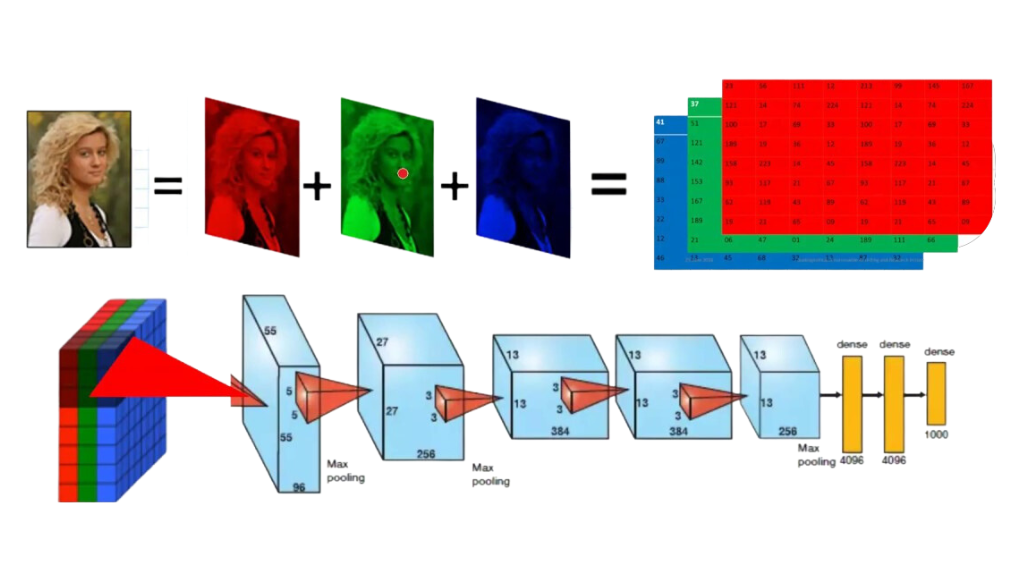
\includegraphics[width=120mm]{fig/classificationimg.png}
        \captionsetup{justification=centering}
	\caption{Phân loại vật thể trong ảnh (nguồn Internet).}
	\label{fig_DlandML}
\end{figure}

Bài toán phân đoạn hình ảnh (image segmentation) là một nhiệm vụ quan trọng trong lĩnh vực thị giác máy tính và xử lý hình ảnh, và nó có vai trò nền tảng trong việc thực hiện bài toán phân loại (classification). Bài toán phân loại sẽ thực hiện nhiệm vụ quyết định đối tượng sẽ thuộc phân lớp nào trong tổng số phân loại đối tượng được nhận diện. Tuy nhiên, để có thể thực hiện chính xác bài toán phân loại, cần phải thực hiện phân đoạn hình ảnh trước đó. 

Phân vùng hình ảnh chia hình ảnh thành các vùng hoặc đối tượng riêng biệt dựa trên các đặc điểm nhận dạng của chúng. Quá trình này giúp xác định vị trí và ranh giới của từng đối tượng trong hình ảnh. Sau khi phân đoạn, mỗi vùng hoặc đối tượng được nhận diện rõ ràng, từ đó có thể áp dụng các kỹ thuật phân loại để đưa ra dự đoán chính xác về phân lớp của từng đối tượng.

Bài toán phân loại sẽ dựa trên đặc điểm nhận dạng của các lớp khác nhau nhằm đưa ra dự đoán chính xác về vật thể \cite{leonard2019image}. Điều kiện tiên quyết để thực hiện được bài toán phân loại vật thể là phải nhận diện được các đối tượng trước từ đó mới dựa trên các đặc điểm của đối tượng để tiến hành phân loại đối tượng.

\section{Mô hình tín hiệu 5G NR và LTE}

Ngày nay, các hệ thống liên lạc qua không trung đóng một vai trò vô cùng quan trọng trong nhiều kịch bản và ứng dụng đa dạng \cite{lin20215g}. Công trình nghiên cứu này chủ yếu tập trung vào các hệ thống thông tin liên lạc 5G NR và LTE. Trên thực tế, các tín hiệu nhận được, hay còn gọi là tín hiệu RX (received signal), từ các nguồn khác nhau có thể được định nghĩa bằng phương trình (\ref{eq:rxsig}). Trong đó, $\mathrm{y(t)}$ biểu thị cho tín hiệu RX, $\mathrm{x(t)}$ là tín hiệu được truyền đi, gọi là tín hiệu TX (transmitted signal), $\mathrm{h(t)}$ đại diện cho đáp ứng kênh, và $\mathrm{n(t)}$ biểu thị cho nhiễu trắng Gaussian cộng thêm (AWGN - Additive white Gaussian noise)

\begin{equation}
    \mathrm{y(t) = x(t) * h(t) + n(t)},
    \label{eq:rxsig}
\end{equation}

\begin{equation}
    \mathrm{Y(\tau, w) = \int_{-\infty}^{\infty} y(t) \cdot w(t - \tau) \cdot e^{-j2\pi ft} \, dt},
    \label{eq:spectrogram}
\end{equation}
\begin{equation}
    \mathrm{E = \sum_{f = f_{\text{min}}}^{f_{\text{max}}} \left| Y(\tau, w) \right|^2}.
    \label{eq:energy}
\end{equation}

\footnotetext[1]{ Toán tử * biễu diễn cho phép nhân chập}


Biến đổi Fourier ngắn hạn (STFT - short-time Fourier transform) là một kỹ thuật xử lý tín hiệu được sử dụng rộng rãi để phân tích nội dung tần số của tín hiệu theo thời gian. Tín hiệu RX (\ref{eq:rxsig}) có thể được biểu diễn trong miền tần số bằng STFT, được định nghĩa trong (\ref{eq:spectrogram}). Cụ thể, $\mathrm{Y(\tau, w)}$ biểu diễn giản đồ phổ của tín hiệu RX tại tần số $\mathrm{f}$ và thời gian $\mathrm{t}$, $\mathrm{y(t)}$ là tín hiệu RX đầu vào, $\mathrm{w(t - \tau)}$ biểu thị hàm cửa sổ được sử dụng để phân đoạn tín hiệu thành các khung ngắn. Hơn nữa, mật độ năng lượng của các mô hình tín hiệu được minh họa bằng phương trình (\ref{eq:energy}), với $E$ biểu thị mật độ năng lượng trong khoảng $\mathrm{\left [ f_{\min}, f_{\max} \right ]}$.

\begin{figure}[h]
    \centering
    \footnotesize
    \begin{tabular}{ccc}
        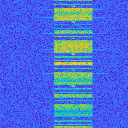
\includegraphics[width=0.25\textwidth]{fig/LTE_frame_0.png}  & 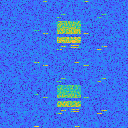
\includegraphics[width=0.25\textwidth]{fig/NR_frame_1506.png} &
        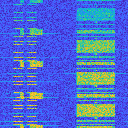
\includegraphics[width=0.25\textwidth]
        {fig/LTE_NR_frame_0.png} 
        \\
        (a) & (b) & (c)
    \end{tabular}
    \caption{Mẫu phổ tín hiệu: (a) LTE, (b) 5G NR, (c) Chồng phổ 5G NR và LTE}
    \label{fig_SignalModel}
\end{figure}

Tỷ lệ tín hiệu trên nhiễu (SNR - signal-to-noise ratio) trong cả hệ thống 5G và LTE có thể được tính toán bằng cách so sánh công suất của tín hiệu với công suất của nhiễu. Trong các hệ thống thông tin liên lạc không dây, SNR thường được định nghĩa là tỷ lệ giữa công suất tín hiệu nhận trung bình và công suất nhiễu trung bình trên một băng thông xác định. Tỷ lệ nhiễu cao hơn có nghĩa là mức độ của các tín hiệu nhiễu không mong muốn so với tín hiệu mong muốn là đáng kể, điều này có thể làm giảm chất lượng và độ tin cậy của việc truyền dữ liệu. Công suất tín hiệu phụ thuộc vào các yếu tố như công suất truyền, suy hao đường truyền, độ lợi của ăng-ten và các hiệu ứng fading. Đặc biệt, có một số mẫu giản đồ phổ trong Hình \ref{fig_SignalModel} trình bày về 5G NR, LTE, và sự chồng lấn giữa 5G và LTE tương ứng.

